\section{Tools}\label{tools}

After reading through the code and documentation of the assignment application, a list of requirements to the web application was compiled.
\\The web application has to:
\begin{enumerate}
	\item Allow input data to be uploaded by an administrator.
	\item Interact with the python application.
	\item Store data persistently in a database.
	\item Visualise the results of the assignment process.
	\item Be accessible over the internet.
	\item Be easy to test and update, via automation.
\end{enumerate}
A virtual machine and an accompanying domain name was provided by SDU for the purpose of hosting the application.\\\\
Following the requirements gathering the next step in the process was to figure out which tools and technologies could be used to build an application fulfilling these requirements. First of all I needed to find a framework in which I could build the application.

\subsection{Framework}

According to Matt Makai in his book Full stack Python \cite{fstack_framework}, ``Frameworks provide functionality in their code or through extensions to perform common operations required to run web applications.''
In essence the framework handles all the underlying functionality of a web application, like URL routing and input form handling. These are functions not imediatly visible to the user. In addition, the framework handles the rendering of templates into dynamic HTML pages, which is what the user sees in their browser.\\\\
Since the web application has to interact closely with the assignment application I decided to use a python framework.\\\\
Of the many \href{https://wiki.python.org/moin/WebFrameworks}{available python web frameworks}, \href{https://www.djangoproject.com/}{Django} and \href{https://flask.palletsprojects.com/en/2.2.x/}{Flask} consistently appeared in every search query I made. According to a survey \cite{framework_survey} made by Stack Overflow, they are also the most widely used python frameworks, which suggests they are robust frameworks, with a high availability of helpful resources.
\begin{figure}[h]
	\begin{tcolorbox}[title={Terminology in regards to python web frameworks},colbacktitle=gray]
		\underline{\textit{View}}:\\A view defines the response to an http request.\\
		\underline{\textit{Template}}:\\A file used to generate the desired content.\\
		\underline{\textit{Decorator}}:\\A way to modify a function by wrapping it in another function.\\
		\underline{\textit{Render}}:\\Turning a template into an HTML page.\\
	\end{tcolorbox}
\label{text:termin_framework}
\end{figure}\\

\subsubsection{Flask}
Flask \cite{Flask_docs} is presented as a minimal framework which only includes the basic functionalities a developer needs to build a website using python \cite{Flask_what}, these basic functionalities mostly consists of routing and rendering.\\
Everything beyond the very basics is performed by 3rd-party extensions, for instance if the developer wants to store data in a database, a Flask application generally relies on an extension for the application to communicate with the database.\\\\
Flask uses a templating language called Jinja2, which allows a developer to write html templates which includes functions with a python like syntax. These functions make it possible to, for example, iterate over a list and for every item in that list, create a component on the page.\\\\
Figures \ref{fig:tools_flask_min} and \ref{fig:tools_flask_min_template} below, shows two simple examples of a Flask application.\\In a Flask application views are defined as functions, and URL routes are defined using decorators such as \verb|@app.route(''/'')|.\\Decorators can also be used to separate views based on HTTP methods, allowing one template to be rendered for a GET request, and another template for a POST request on the same URL.
\begin{figure}[b!]
\centering
\hrule
\vspace*{0.2cm}
%\begin{minipage}{.4\textwidth}
%\centering
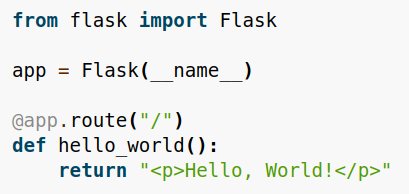
\includegraphics[width=.4\textwidth]{flask_minimal}
\caption{An example of a very simple Flask application, in which a user is presented with a simple page showing ``Hello, World!'' when navigating to the URL ``/''.}
\label{fig:tools_flask_min}
%\end{minipage}%
%\hspace{1cm}
%\begin{minipage}{.4\textwidth}
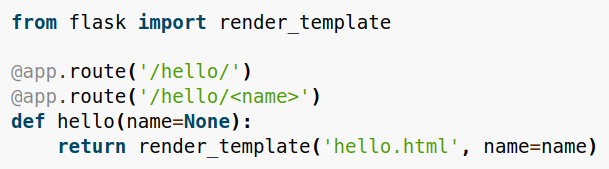
\includegraphics[width=.4\textwidth]{flask_minimal_template}
\caption{An example of a minimal flask application using templates, in which a user is shown the contents of ``hello.html'' when navigating to ``/hello/'' or\\``/hello/<name>''.}
\label{fig:tools_flask_min_template}
%\end{minipage}
% \hrule
\end{figure}
\\\\
With regards to security in a Flask application \cite{Flask_security} only cross-site scripting is prevented, and only when HTML pages are generated using Jinja2. Cross-site scripting \cite{owasp_xss} is a type of attack where a malicious party executes malicious code on a user's computer, through a vulnerable website. Other types of attacks such as cross site request forgery \cite{owasp_csrf} where a forged request is send to a user, forcing the user user to perform an action on the website, are handled by extensions. Management of http request headers, including security headers, are handled by yet another extension.
\\\\
The reliance of extensions allows a developer building a Flask application to only include the functionalities needed for that particular application. This approach means the application will indeed be minimal, however it might complicate the development process when the developer has to find the right or best extension to perform a given task.

\subsubsection{Django}
Django is presented as a framework that includes everything needed to develop a web application ``from concept to completion as quickly as possible'' \cite{Django_home}.
Django includes an object-relational mapper (ORM) which allows a developer to define a relational database as a collection of python classes, illustrated in Figure \ref{fig:tools_django_models}, and makes it possible to write queries as python expressions instead of SQL statements. 
\begin{figure}[b!]
\centering
\hrule
\vspace*{0.2cm}
%\begin{minipage}{.5\textwidth}
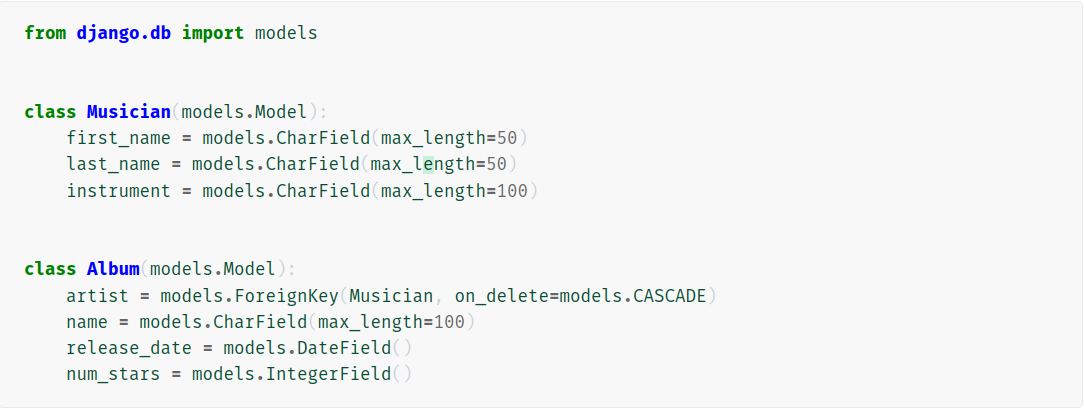
\includegraphics[width=.6\textwidth]{django_models}
\caption{An example from the Django documentation of a simple database with two tables, Musician and Album.}
\label{fig:tools_django_models}
%\end{minipage}%
%\hspace{1cm}
%\begin{minipage}{.5\textwidth}
%\centering
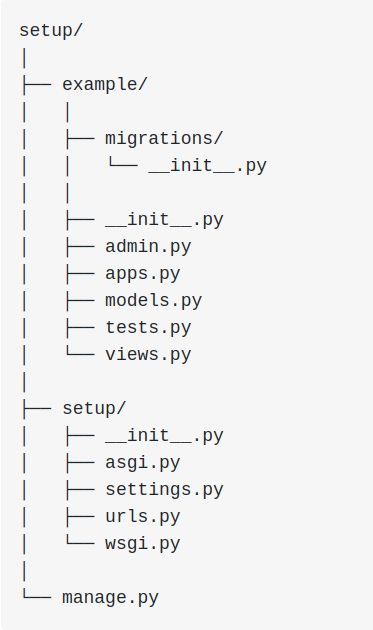
\includegraphics[scale=0.35]{django_structure}
\caption{An example of the default folder structure of a Django project.}
\label{fig:tools_django_structure}
% \hrule
%\end{minipage}
% \hrule
\end{figure}
Django officially supports five different databases, PostgreSQL, MariaDB, MySQL, Oracle and SQLite \cite{Django_db}, extensions can be installed to add support for other databases if needed. Django automatically creates an admin page from which entries in the database can be created, deleted and edited.\\\\
Django natively supports two templating languages, Jinja2 and Django templating language, they use a very similar syntax \cite{DTL_to_jinja}, Jinja2 being inspired by Django\footnote{Mentioned briefly in the jinja2 \href{https://jinja.palletsprojects.com/en/3.1.x/templates/}{documentation}}.\\\\
Views in Django, like in Flask, are generally written as functions, however class based views, where views are instead written as python classes are supported. URL routing is handled in a separate file, \verb|urls.py|, in which a URL is mapped to a view function.\\\\
By default projects made using Django is organized in a predefined folder structure, automatically created by Django, illustrated in Figure \ref{fig:tools_django_structure}.\\\\
Protection against several kinds of attacks, such as cross site scripting, cross site request forgery and SQL injections are included in Django by default.\\\\
The everything-included approach of Django allows a developer to build a web application by ``filling in the blanks'', this approach does however limit the freedom of the developer to choose which components to include.\\In the podcast ``Talk python to me'' episode 149 \cite{talk_python} at timestamp 40:24, Nicholas Hunt-Walker summarizes the approach as follows: ``...it encourages rapid development as long as you want to do things the Django way, which is oftentimes a good way to do things, but if you want to go outside that norm, you're going to have to pull apart some code to do that.''\\\\
I decided to use the Django framework because the features it includes is a good fit for this project.


\subsection{Persistent data}
After deciding on a framework, the next step was to make a decision on which type of database to use. I found that the book Full Stack Python \cite{which_db} was a great resource for finding information about commonly used relational databases, in particular MySQL, PostgreSQL and SQLite which are all supported by Django.\\\\
SQLite support is built in to python \cite{python_sqlite} enabling communication between the python application and the database without further configuration, while MySQL and PostgreSQL both require the inclusion of a separate driver libraries to facilitate communication.\\
SQLite is the default when starting a new Django project, changing to another supported database is however well documented and several step-by-step guides exists\footnote{How to connect mySQL to django: \\\tiny\url{https://www.javatpoint.com/how-to-connect-mysql-to-django}}$^{,}$\footnote{How to Start Django Project with a Database(PostgreSQL):\\\tiny\url{https://stackpython.medium.com/how-to-start-django-project-with-a-database-postgresql-aaa1d74659d8}}.\\
MySQL and PostgreSQL both work by having their own separate server processes which handle reads and writes to the database. The reliance on this server process makes it possible to have the database running on a remote host machine, allowing several applications, or multiple instances of the same application, to use the same database while not necessarily running on the same machine.\\
Access to a MySQL or PostgreSQL Database is restricted to only allow authorized users, or processes, to read and/or write to the database.\\
SQLite on the other hand relies on the file system of the host machine to perform reads and writes directly to an ordinary file. This approach limits the access to an SQLite database to processes running on the host machine, with no way of controlling the access to the file besides the access control provided by the host operating system.\\\\
When choosing a database for a web application a major consideration is the concurrency aspect, a user should be able to read from and write to the database without disrupting the work of other users of the application.\\
With concurrency in mind, the Django documentation advises against the use of SQLite \cite{Django_db_lock}, in an environment with many concurrent operations involving the database. Strategies do however exists to reduce the likelihood of concurrency errors, like increasing the timeout value and using the Write-Ahead logging mode \cite{SQLite_testing,SQLite_wal}.\\Considering the expected number of users is well within the range of what the SQLite documentation calls ``low to medium'' while also stating that ``Generally speaking, any site that gets fewer than 100K hits/day should work fine with SQLite'' \cite{sqlite_when}, and since support for it is build into python I decided to use SQLite as the database for the application.\\The extra work required to use either MySQL or PostgreSQL, was deemed unnecessary since SQLite would be sufficient for this project.

